\section{Implementation of Core Functionalities}

This project contains 3 componets work togather in order to makeup the entire system. In this section the inner working of each of those components will be explained.

\subsection{Lazy-Koala Operator}

Lazy-Koala operator is the heart of the entire project which is responsible for binding all other components together. In the context of Kubernetes, an operator is an agent that's running on the cluster which is responsible for keeping one or more dedicated resources in sync with the desired state. 

For example, Kubernetes has a built-in resource named "Pod" which is the smallest deployable object in Kubernetes. So when a system administrator asked the Kube-API to create a pod out of a certain Docker container, Kube-API will create a resource object and attach it to the operator. Once that's done the pod operator will parse the pod resource specification and pod out of it. If for some reason the pod crashes or the administrator change the specification of the pod, the operator will be notified and it will run its reconciliation function to match the observed state with the desired state.

Coming back to the Lazy-Koala operator, it has a Custom Resource Definition (CRD) called inspector. In its specification, there are three required values. Deployment reference, DNS reference, and an URL to download the model that was fine-tuned for this specific deployment. So once a resource was deployed, the operator will first get the Pods related to the deployment and populate the "scrapePoints" data structure
with the IP of each of those. Then it's going to find out the IP address mapped to the DNS reference append that to the "scrapePoints". Then the operator will append all the scrapePoints to ConfigMap which was deployed as part of the installation process. This ConfigMap gets mounted to every Gazer instance via Kubernetes volumes system so the change here will instantly be reflected with the Gazer instances. As a final step, an instance of Sherlock will be provisioned with the model given in the specification.

Figure \ref{fig:reconcile-loop} shows a part of this reconciliation loop, which get repeated every time there is a change to an existing resource or whenever the user creates a new variant of this resource.

\begin{figure}[H]
    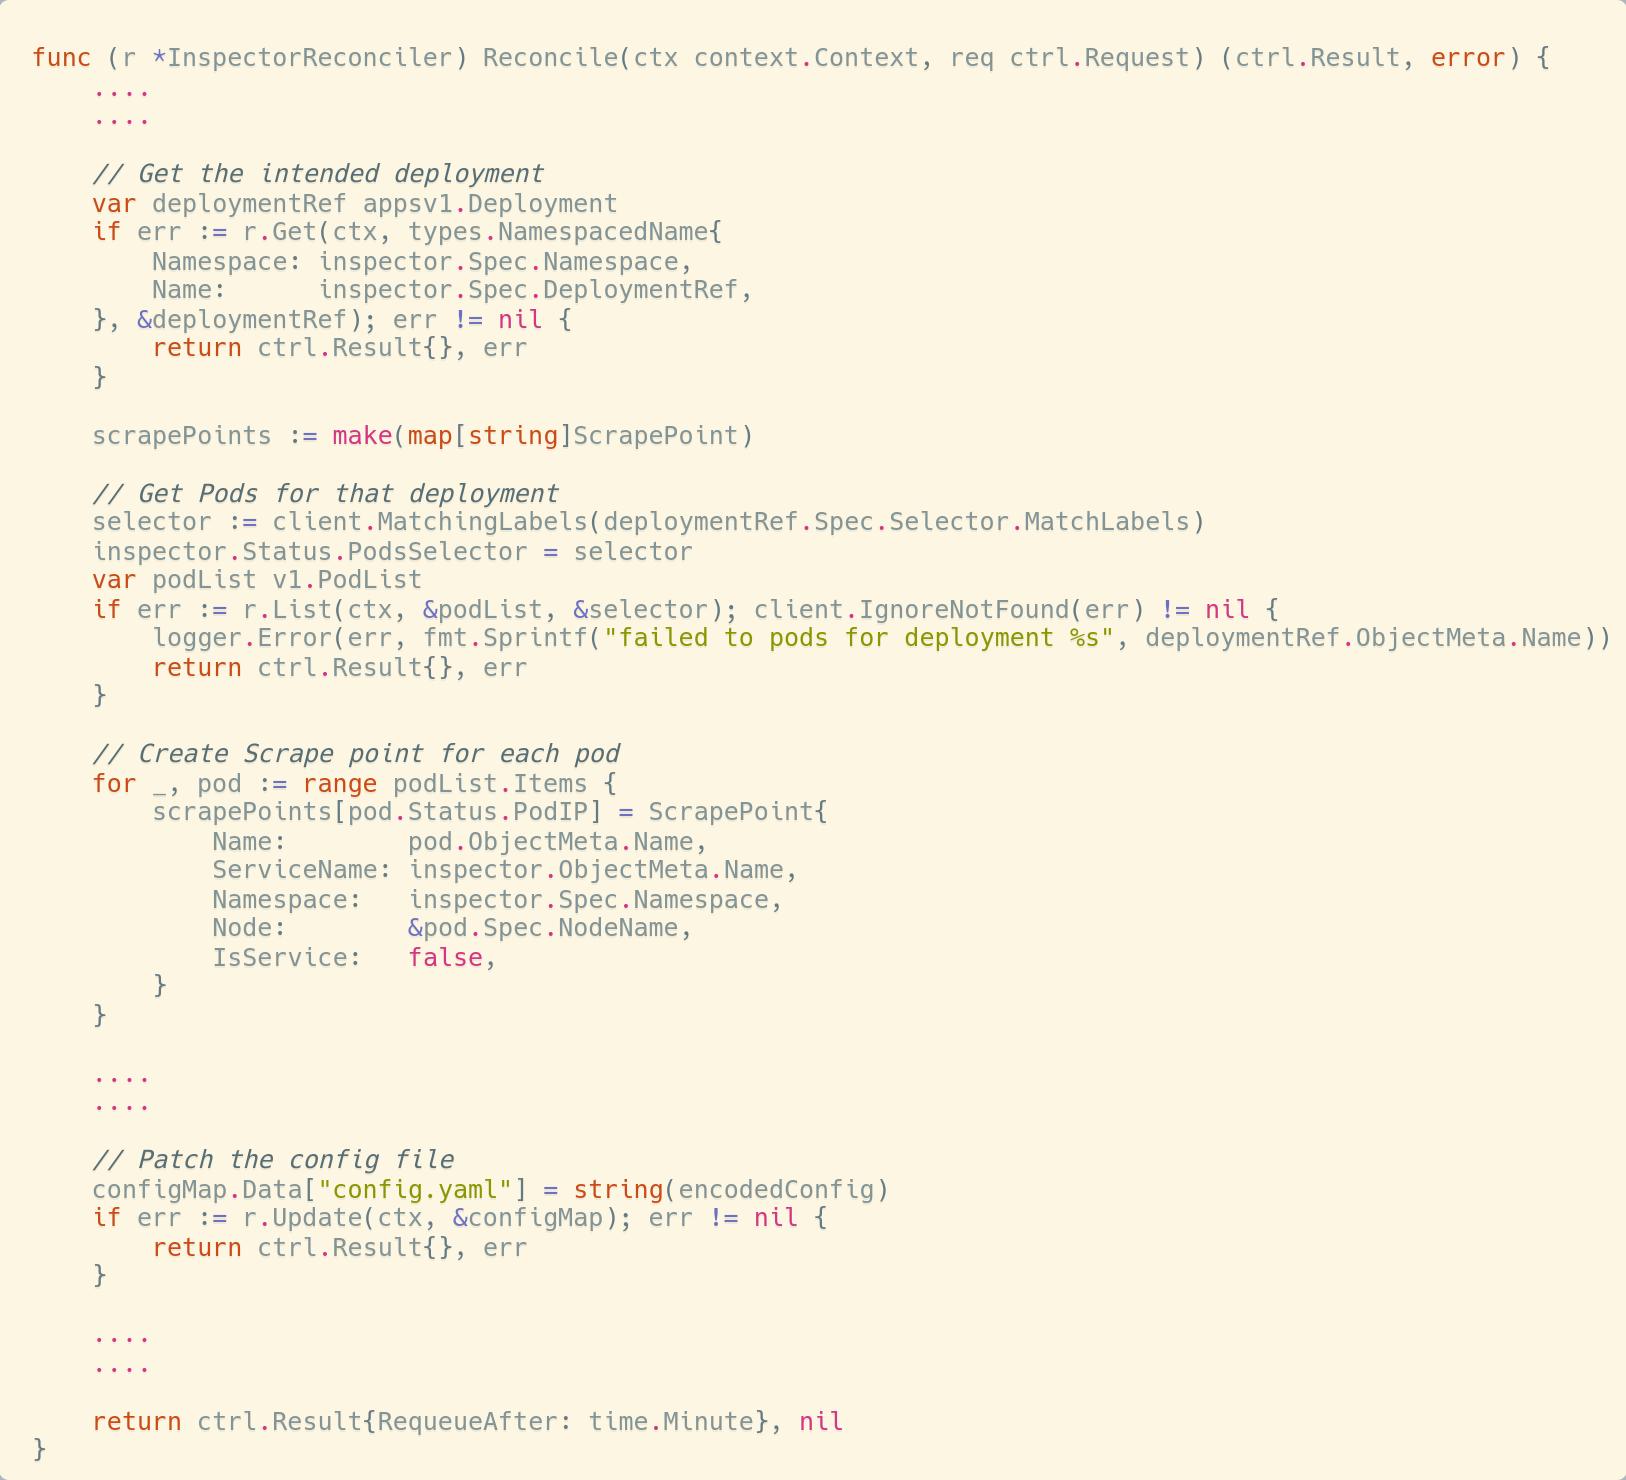
\includegraphics[height=11.5cm]{assets/implementation/reconcile-loop.png}
    \caption{Operator Reconciliation Loop (self-composed)}
    \label{fig:reconcile-loop}
\end{figure}



\subsection{Gazer}

Gazer is the telemetry exraction agent

\begin{figure}[H]
    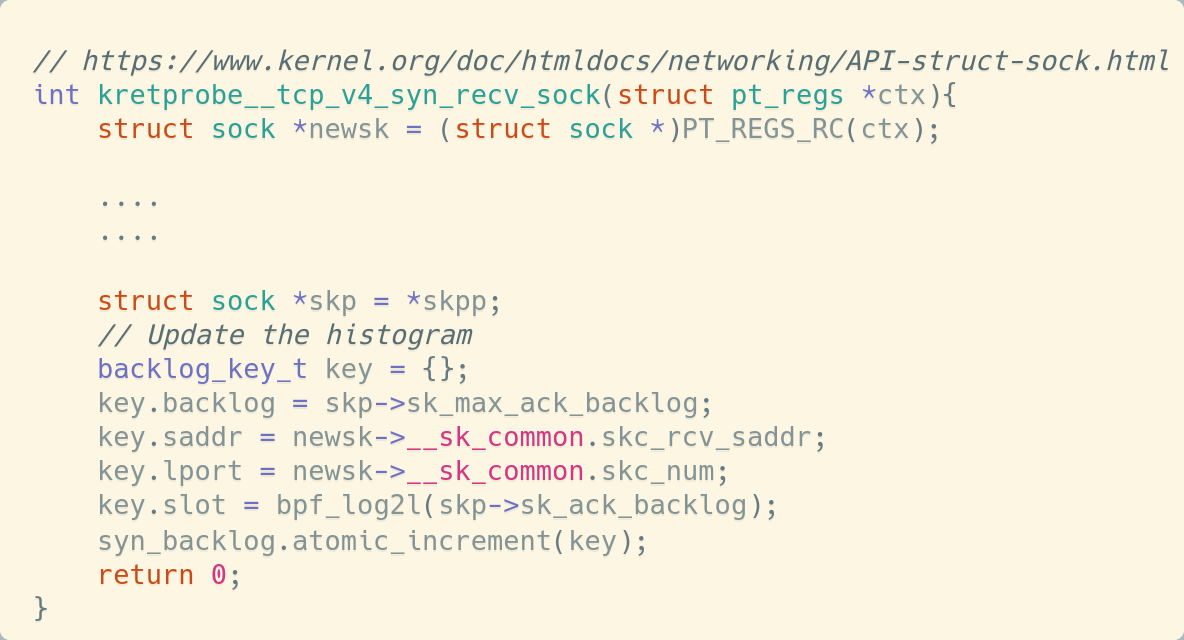
\includegraphics[width=14cm]{assets/implementation/backlog-probe.png}
    \caption{\ac{ebpf} probe to collecting tcp backlog (self-composed)}
    \label{fig:backlog-probe}
\end{figure}





\subsection{Sherlock}

\begin{figure}[H]
    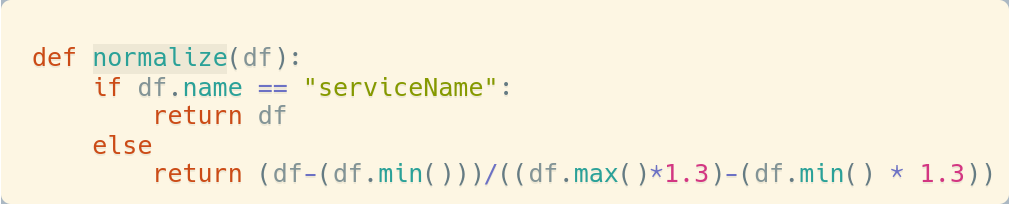
\includegraphics[width=14cm]{assets/implementation/normalize-data.png}
    \caption{Data normalization function (self-composed)}
    \label{fig:normalize-data}
\end{figure}


\begin{figure}[H]
    \centering
    \begin{subfigure}[b]{0.48\textwidth}
        \centering
        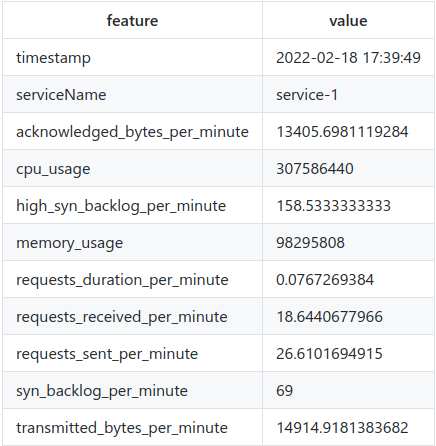
\includegraphics[width=\textwidth]{assets/implementation/before-normalization.png}
        \caption{Before Normalization}
        \label{fig:before-normalization}
    \end{subfigure}
    \hfill
    \begin{subfigure}[b]{0.49\textwidth}
        \centering
        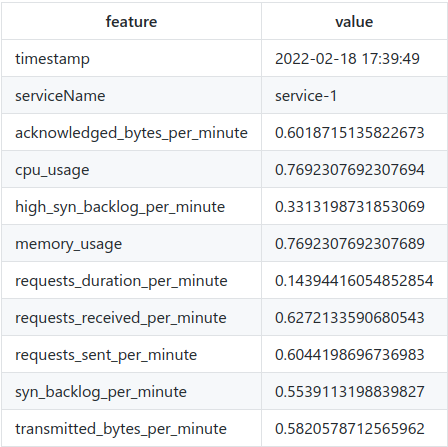
\includegraphics[width=\textwidth]{assets/implementation/after-normalization.png}
        \caption{After Normalization}
        \label{fig:after-normalization}
    \end{subfigure}
    \hfill
       \caption{Comparsion of a data point before and after normalization (self-composed)}
\end{figure}

\begin{figure}[H]
    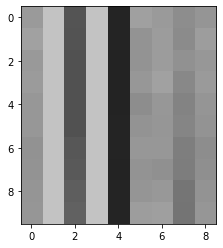
\includegraphics[width=7cm]{assets/implementation/visualize-representation.png}
    \caption{Visualization of encoded time series (self-composed)}
    \label{fig:visualize-representation}
\end{figure}
